\chapter{Time integration}\label{ch:time}

The equations of \cref{ch:eq} carry two kinds of motion with very different speeds:
\begin{itemize}
  \item the meteorologically important flow, advected at tens of metres per second;
  \item acoustic waves, at about 340~m/s.
\end{itemize}
A time step small enough for sound would waste most of its work on slow processes. WRF therefore splits the
integration \citep{wicker2002,klemp2007}:
\begin{itemize}
  \item a third-order Runge--Kutta (RK3) scheme integrates the slow terms with the large step $\Delta t$;
  \item inside each RK stage, a forward--backward scheme integrates the acoustic terms with small steps $\Delta\tau$;
  \item a vertically implicit solve removes the vertical acoustic limit, which on thin layers near the ground would
    be the most severe.
\end{itemize}
All of this happens in \src{dyn_em/solve_em.F}{solve_em}, one call per domain per large step.

\section{The Runge--Kutta scheme}

For a prognostic variable $\Phi$ with slow tendency $R(\Phi)$, the RK3 step from $t$ to $t + \Delta t$ is
\begin{align}
  \Phi^{*}  &= \Phi^{t} + \frac{\Delta t}{3}\,R(\Phi^{t}), \notag\\
  \Phi^{**} &= \Phi^{t} + \frac{\Delta t}{2}\,R(\Phi^{*}), \label{eq:rk3}\\
  \Phi^{t+\Delta t} &= \Phi^{t} + \Delta t\,R(\Phi^{**}). \notag
\end{align}
It is third-order accurate for linear equations and second order for non-linear ones. With the fifth-order
upwind-biased advection of \cref{ch:adv}, it is stable up to an advective Courant number of about 1.4
\citep{wicker2002}. Every stage starts from $\Phi^t$; only the tendency changes. In the code the loop is
\code{Runge_Kutta_loop: DO rk_step = 1, rk_order}, and the stage length is \code{dt_rk}: $\Delta t/3$,
$\Delta t/2$ and $\Delta t$.

\section{Acoustic sub-steps}

Within each RK stage, the acoustic and gravity-wave terms are integrated from $t$ to $t + \mathrm{dt\_rk}$ in small
steps. The number of small steps per full $\Delta t$, $n_s$, is \code{time_step_sound}. When the namelist leaves it
at 0, \code{solve_em} computes it from the grid spacing $\Delta x$ and the largest map factor:
\begin{equation}
  n_s = \max\!\Bigl(2\,\Bigl(\Bigl\lfloor \frac{300\,\Delta t}{\Delta x / m_{\max}} - 0.01 \Bigr\rfloor + 1\Bigr),\; 4\Bigr),
  \qquad \Delta\tau = \Delta t / n_s .
\end{equation}
Both domains of the case have $300\,\Delta t/\Delta x = 1$, so $n_s = 4$. The three stages then take:
\begin{center}
\begin{tabular}{lccc}
\toprule
Stage & \code{dt_rk} & small steps & small step \code{dts_rk} \\
\midrule
1 & $\Delta t/3$ & 1 & $\Delta t/3$ \\
2 & $\Delta t/2$ & $n_s/2 = 2$ & $\Delta\tau$ \\
3 & $\Delta t$ & $n_s = 4$ & $\Delta\tau$ \\
\bottomrule
\end{tabular}
\end{center}
That is seven acoustic sub-steps per large step, each launching a sequence of kernels on the GPU
(\cref{ch:fusion}).

\begin{figure}[ht]
\centering
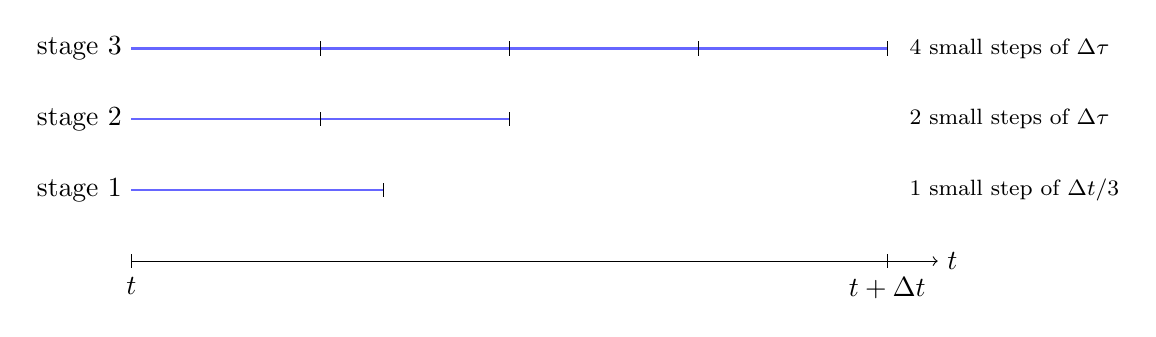
\begin{tikzpicture}[x=1.6cm,y=0.9cm]
  \draw[->] (0,0) -- (6.4,0) node[right] {$t$};
  \foreach \x/\l in {0/$t$, 6/$t+\Delta t$} { \draw (\x,0.1) -- (\x,-0.1) node[below] {\l}; }
  \draw[thick, blue!60] (0,1) -- (2,1); \node[left] at (0,1) {stage 1};
  \draw (2,1.1) -- (2,0.9);
  \draw[thick, blue!60] (0,2) -- (3,2); \node[left] at (0,2) {stage 2};
  \foreach \x in {1.5,3} { \draw (\x,2.1) -- (\x,1.9); }
  \draw[thick, blue!60] (0,3) -- (6,3); \node[left] at (0,3) {stage 3};
  \foreach \x in {1.5,3,4.5,6} { \draw (\x,3.1) -- (\x,2.9); }
  \node[right, font=\footnotesize] at (6.1,1) {1 small step of $\Delta t/3$};
  \node[right, font=\footnotesize] at (6.1,2) {2 small steps of $\Delta\tau$};
  \node[right, font=\footnotesize] at (6.1,3) {4 small steps of $\Delta\tau$};
\end{tikzpicture}
\caption{The time-split RK3 step with $n_s = 4$. Every stage integrates from $t$, with the slow tendency of the
previous stage held fixed; the tick marks are acoustic sub-steps.}
\label{fig:rk3}
\end{figure}

\subsection{The acoustic variables}

The small steps advance deviations from the state at the start of the large step. For each prognostic variable the
code forms, in \src{dyn_em/module_small_step_em.F}{small_step_prep},
\begin{equation}
  U'' = U - U^{t},\quad V'' = V - V^{t},\quad W'' = W - W^{t},\quad
  \Theta'' = \Theta - \Theta^{t},\quad \mu'' = \mu_d - \mu_d^{t},\quad \phi'' = \phi - \phi^{t}.
\end{equation}
The slow tendencies $R_U, R_V, \dots$, computed once per stage from the latest RK state (\cref{alg:solve-em}),
are held fixed during the stage. The acoustic equations are the linearized pressure-gradient, divergence and
buoyancy terms of \cref{eq:U,eq:V,eq:W,eq:T,eq:mu,eq:phi}.

\subsection{Forward--backward sequence}

Each small step $\tau \to \tau + \Delta\tau$ updates the variables in a fixed order (\cref{alg:small-step}):
\begin{enumerate}
  \item The pressure is diagnosed from the current $\theta''$, $\mu''$ and $\phi''$
    (\src{dyn_em/module_small_step_em.F}{calc_p_rho}), and a divergence damping is added to it:
    \begin{equation}
      p''_{\mathrm{damp}} = p'' + \gamma_d\,\bigl(p'' - p''_{\tau-\Delta\tau}\bigr), \qquad \gamma_d = \mathrm{smdiv}
      \ (0.1 \text{ by default}).
    \end{equation}
  \item $U''$ and $V''$ are stepped forward with the pressure gradient of that pressure
    (\src{dyn_em/module_small_step_em.F}{advance_uv}). An external-mode filter, weighted by \code{emdiv}, damps the
    fast mode of the column mass.
  \item With the new horizontal fluxes, the column mass $\mu''$, the vertical mass flux $\Omega''$ and $\Theta''$ are
    updated (\src{dyn_em/module_small_step_em.F}{advance_mu_t}). Integrating \cref{eq:mu} from the surface gives
    $\Omega''$ level by level.
  \item $W''$ and $\phi''$ are solved together, implicitly in the vertical
    (\src{dyn_em/module_small_step_em.F}{advance_w}).
\end{enumerate}
The new horizontal momentum is used in the continuity equation within the same small step (\emph{backward}), which
is what makes the scheme stable for acoustic waves.

\subsection{Off-centering}

The vertically implicit terms are weighted toward the new time level by the off-centering parameter
$\beta = \mathrm{epssm}$:
\begin{equation}
  \overline{\psi}^{\tau} = \frac{1+\beta}{2}\,\psi^{\tau+\Delta\tau} + \frac{1-\beta}{2}\,\psi^{\tau}.
\end{equation}
The code writes this average in the same form, for example
\code{t_2ave = .5*((1.+epssm)*t_2 + (1.-epssm)*t_2ave)} in \code{advance_w}, and
\code{MUAVE = .5*((1.+epssm)*MU + (1.-epssm)*MUAVE)} in \code{advance_mu_t}. $\beta > 0$ damps vertically
propagating sound waves. The case uses 0.5 on d01 and 0.8 on d02, larger than the default 0.1, because of the steep
terrain.

\section{The vertically implicit solve}

Eliminating $\phi''$ from the coupled $w$--$\phi$ equations of the small step gives, in every column, a tridiagonal
system for $W''$ on the full levels $k = 2, \dots, n_z - 1$ (the surface value comes from the terrain-following
boundary condition and the top value from the lid condition):
\begin{equation}
  a_k\,W''_{k-1} + b_k\,W''_k + c_k\,W''_{k+1} = r_k .
\end{equation}
The coefficients depend only on the base state and the stage's column mass, so they are computed once per RK stage
by \src{dyn_em/module_small_step_em.F}{calc_coef_w}. With
$\kappa = \bigl(\tfrac12\,\Delta\tau\, g\,(1+\beta)\bigr)^2$ (\code{cof}) and $c^2_a = \gamma\,p/\alpha$
(\code{c2a}, set in \code{small_step_prep}), they are
\begin{align}
  a_k &= -\,\kappa\; q_{w,k}\; \frac{c^2_{a,k-1}}{\Delta\eta_{k-1}\,\Delta\eta_{f,k}\;\mu_{h,k-1}\,\mu_{f,k-1}}, \notag\\
  b_k &= 1 + \kappa\; q_{w,k}\; \frac{1}{\Delta\eta_{f,k}}
         \left(\frac{c^2_{a,k}}{\Delta\eta_k\,\mu_{h,k}\,\mu_{f,k}} + \frac{c^2_{a,k-1}}{\Delta\eta_{k-1}\,\mu_{h,k-1}\,\mu_{f,k}}\right), \\
  c_k &= -\,\kappa\; q_{w,k}\; \frac{c^2_{a,k}}{\Delta\eta_k\,\Delta\eta_{f,k}\;\mu_{h,k}\,\mu_{f,k+1}}, \notag
\end{align}
where $q_{w}$ is the moisture factor \code{cqw}, $\Delta\eta_k$ is the thickness of layer $k$ (\code{1/rdnw}),
$\Delta\eta_{f,k}$ the distance between the half levels around full level $k$ (\code{1/rdn}), and $\mu_h$, $\mu_f$
are the metrics $c_1\mu + c_2$ on half and full levels. The indices are those of the code, including the full-level
metric of level $k-1$ in $a_k$. The first row has $a_2 = 0$, and the top row ($k = n_z$) has its own coefficients
from the lid condition. The code stores the forward-elimination factors $\alpha_k$ and $\gamma_k$, so each small step only
performs the two sweeps.

\begin{algorithm}[ht]
\caption{The tridiagonal solve for $W''$ in one column. \code{calc_coef_w} computes the factors once per stage;
\code{advance_w} performs the two sweeps every small step.}
\label{alg:tridiag}
\begin{algorithmic}[1]
\State \textbf{once per stage} (\code{calc_coef_w}):
\State $\gamma_1 \gets 0$
\For{$k = 2, \dots, n_z - 1$} \Comment{upward recurrence}
  \State $\alpha_k \gets 1 / (b_k - a_k\,\gamma_{k-1})$; \quad $\gamma_k \gets c_k\,\alpha_k$
\EndFor
\State \textbf{every small step} (\code{advance_w}):
\For{$k = 2, \dots, n_z$} \Comment{forward sweep, bottom up}
  \State $W''_k \gets (W''_k - a_k\,W''_{k-1})\,\alpha_k$
\EndFor
\For{$k = n_z - 1, \dots, 2$} \Comment{back substitution, top down}
  \State $W''_k \gets W''_k - \gamma_k\,W''_{k+1}$
\EndFor
\end{algorithmic}
\end{algorithm}

After the solve, \code{advance_w} applies the upper Rayleigh damping of $w$ (\code{damp_opt = 3}, \cref{ch:turb})
and recovers $\phi''$ from the updated $W''$, from the top down.

\begin{portnote}
\Cref{alg:tridiag} is a recurrence in $k$: each level needs the previous one. On the GPU the parallelism is across
columns, one thread per $(i,j)$, and each thread runs the sweeps in the original order (Template C, kernels K-CCW and
K-AW, \cref{ch:port}). The CPU code loops over $j$ outside, $k$ in the middle and $i$ inside, so for a fixed $j$ it
holds a whole $(i,k)$ slab of temporaries. On the GPU those slabs become private arrays of one column each. Only
the indices change, not the arithmetic.
\end{portnote}

\section{Time-averaged fluxes and the end of the small steps}

Scalars (moisture, TKE) are not advanced in the acoustic loop. They are transported once per RK stage with mass
fluxes averaged over the stage's small steps, so that they are consistent with the mass continuity of the acoustic
integration. \src{dyn_em/module_small_step_em.F}{sumflux} accumulates $\overline{U}$, $\overline{V}$ and
$\overline{\Omega}$ over the small steps. \src{dyn_em/module_small_step_em.F}{small_step_finish} then turns the
acoustic variables back into full ones:
\begin{itemize}
  \item it adds the stage's start values;
  \item it divides the coupled fields by the new column mass.
\end{itemize}

\section{One step of solve\_em}

\begin{algorithm}[ht]
\caption{One large step of \code{solve_em} for one domain (simplified; the case's options). Physics and fire are
called inside RK stage 1, before the slow tendencies are formed.}
\label{alg:solve-em}
\begin{algorithmic}[1]
\For{$\mathrm{rk\_step} = 1, 2, 3$}
  \State prepare the stage: couple momentum, $\Omega$, moisture factors (\code{rk_step_prep}); physical boundaries
  \If{$\mathrm{rk\_step} = 1$}
    \State physics: radiation, surface, PBL, fire (\code{first_rk_step_part1}); diffusion metrics, TKE (\code{first_rk_step_part2})
  \EndIf
  \State slow tendencies: advection, pressure gradient, buoyancy, Coriolis, curvature, mixing (\code{rk_tendency})
  \State lateral boundaries: relaxation and specified zones (\code{relax_bdy_dry}, \code{spec_bdy_dry}); add physics tendencies (\code{rk_addtend_dry})
  \State \code{small_step_prep}; \code{calc_p_rho} (step 0); \code{calc_coef_w}
  \For{each small step of the stage}
    \State \cref{alg:small-step}
  \EndFor
  \State \code{small_step_finish}
  \State scalars: advection with the averaged fluxes; positive-definite in the last stage (\code{rk_scalar_tend}, \code{rk_update_scalar(_pd)})
  \State boundaries of scalars; \code{calc_p_rho_phi}; physical boundaries (\code{rk_phys_bc_dry_2})
\EndFor
\State microphysics (\code{microphysics_driver}) and its coupling (\code{moist_physics_prep_em}, \code{moist_physics_finish_em})
\end{algorithmic}
\end{algorithm}

\begin{algorithm}[ht]
\caption{One acoustic sub-step (inside \code{small_steps}).}
\label{alg:small-step}
\begin{algorithmic}[1]
\State $p''$ with divergence damping (\code{calc_p_rho})
\State $U''$, $V''$ forward (\code{advance_uv}); specified-zone updates (\code{spec_bdyupdate})
\State $\mu''$, $\Omega''$, $\Theta''$ (\code{advance_mu_t}); specified-zone updates
\State $W''$, $\phi''$ implicitly (\code{advance_w}, \cref{alg:tridiag}); boundary updates (\code{spec_bdyupdate_ph}, \code{zero_grad_bdy})
\State accumulate averaged fluxes (\code{sumflux})
\end{algorithmic}
\end{algorithm}

\begin{portnote}
On the GPU every call in \cref{alg:solve-em,alg:small-step} becomes one or more kernels. Per d02 step that is several
hundred launches, about half of them in the seven acoustic sub-steps. The arithmetic of each kernel is small, so the
launch overhead and the many reads and writes of the same fields between kernels matter. This makes the acoustic
loop the first target of kernel fusion (\cref{ch:fusion}).
\end{portnote}
